\section{Project Results}

% \subsection{Upgrade Dependencies}
% 
% \begin{frame}[c]
%     From Django 2 to Django 3 \\
%     (Django 4 released during the project, has been decided to go to 3 in production first) \\
%     Now requires \mintinline{python}{DEFAULT_AUTO_FIELD = "django.db.models.AutoField"}
% \end{frame}

\subsection{Proper Logging}

\begin{frame}[c]{Changes to Logging}
    \large
    \begin{itemize}[<+(1)->]
        \item Logging used to be over individual `print` statements
        \item Properly defined Logging levels (debug, info, warn, error, critical)
        \item Logging to console, syslog and file
        \item Differing formatter for console and other (timestamps, ...)
        \item Rotating files: Keep last five days, overwrite after
    \end{itemize}
\end{frame}

\begin{frame}[c]{Logging Before: Example} 
    \todo{Screenshot: Logging before, Optional}
\end{frame}

\pic{Logging Now: Example}{33}

\subsection{Automatically generate Documentation}

\begin{frame}[c]{Why is this worth trying?} 
    \begin{itemize}[<+(1)->]
        \item 
    \end{itemize}
\end{frame}

\begin{frame}[c]{Automatically Generate Documentation}
    \begin{multicols}{2}
        \large
        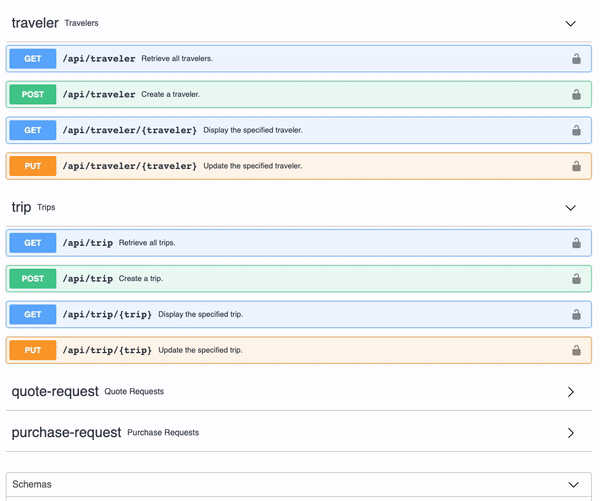
\includegraphics[width=0.5\textwidth]{swagger} \\
        (Example) \\
        Failed, because:
        \begin{itemize}[<+(1)->]
            \item Mainly used to generate documentation for JSON endpoints
            % \item Few comments to generate documentation from
            \item 'Primitive' Views lacking important information for automatic generation
        \end{itemize}
        Was worth a try.
    \end{multicols}
\end{frame}

\subsection{What Research is the Storage used for?}

\begin{frame}[c]{What Research is the Storage used for?}
    \begin{multicols}{2}
    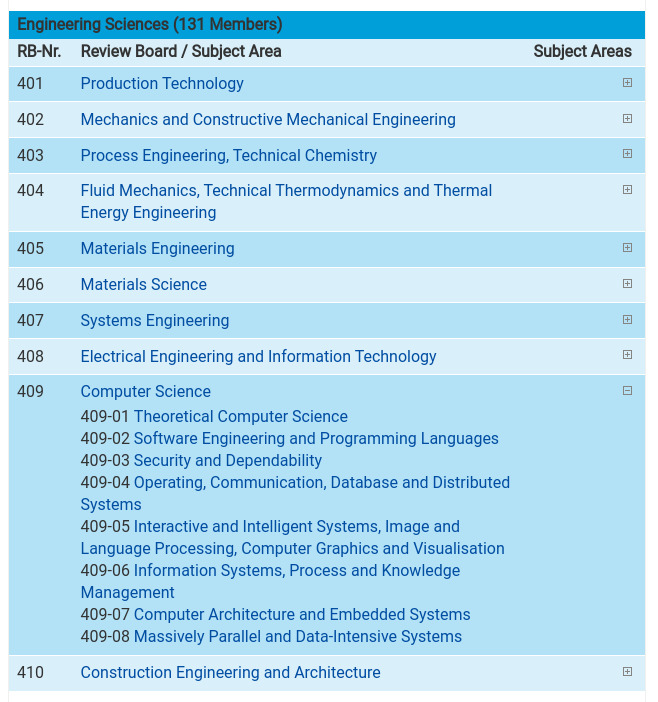
\includegraphics[width=0.5\textwidth]{Selection_032}
    \large
        \begin{itemize}[<+(1)->]
            \item We want to know more about our users
            \item This includes affiliation of research projects
            \item Good separation in subject areas from 'Deutsche Forschungsgesellschaft'
        \end{itemize}
    \end{multicols}
\end{frame}

\pic{Selection of DFG Subject Area upon Project Creation}{10}

\begin{frame}[c]{Selection of DFG Discipline}
    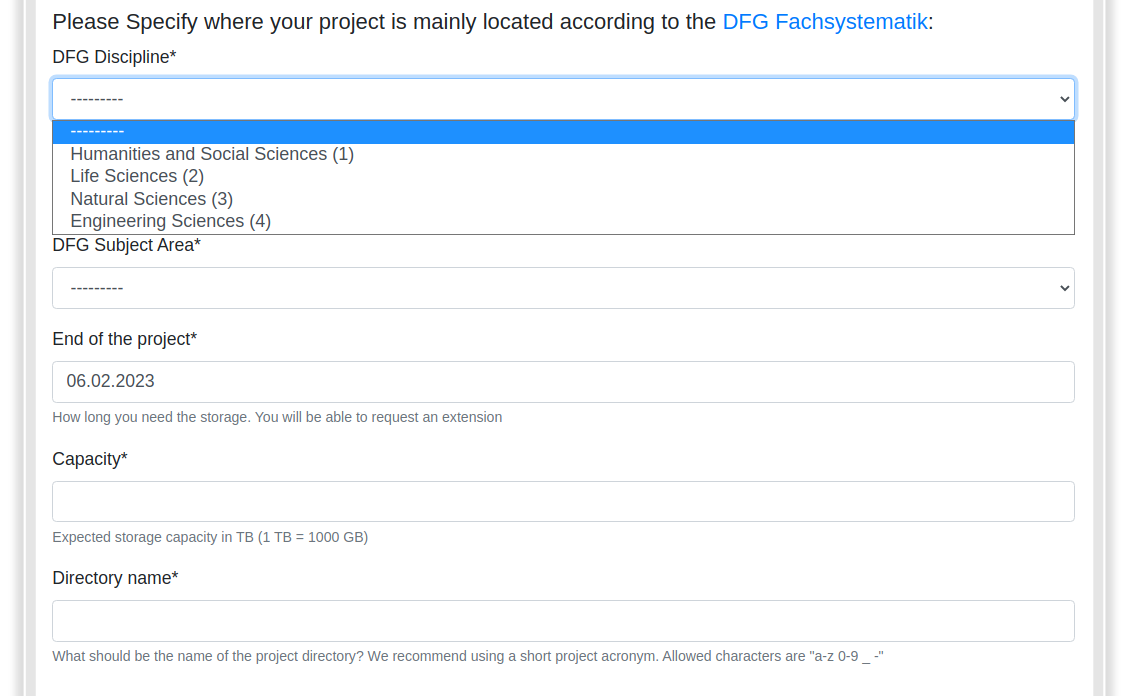
\includegraphics[width=\textwidth]{select_discipline}
\end{frame}
\begin{frame}[c]{Selection of DFG Subject without Board}
    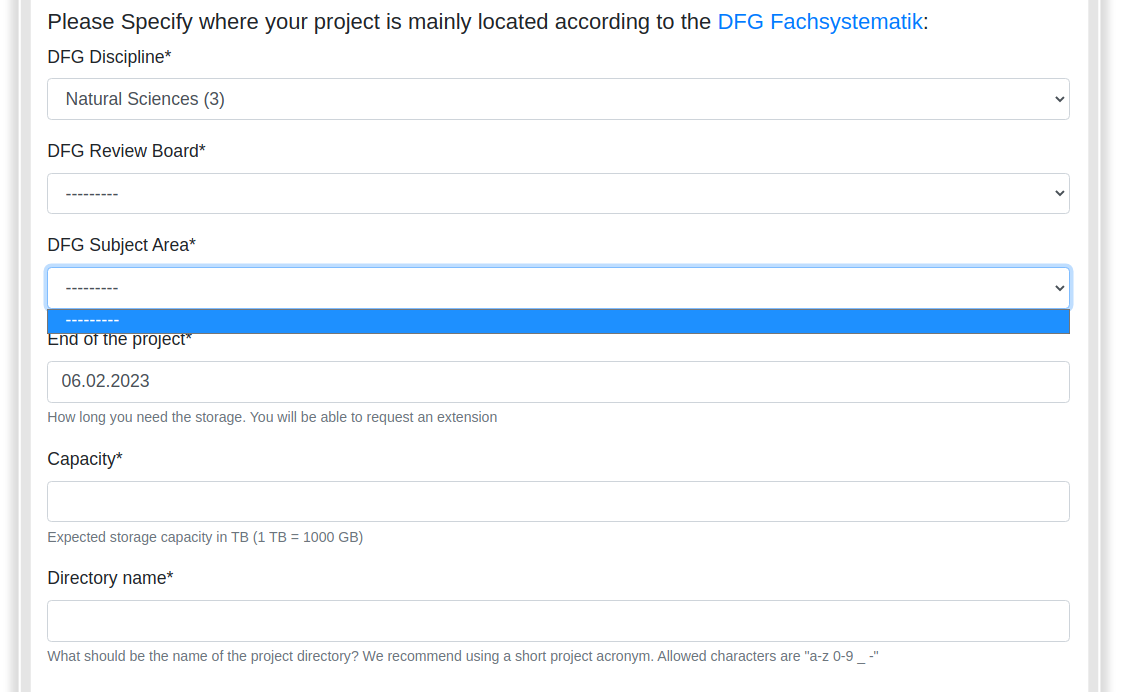
\includegraphics[width=\textwidth]{select_subject1}
\end{frame}
\begin{frame}[c]{Selection of DFG Subject}
    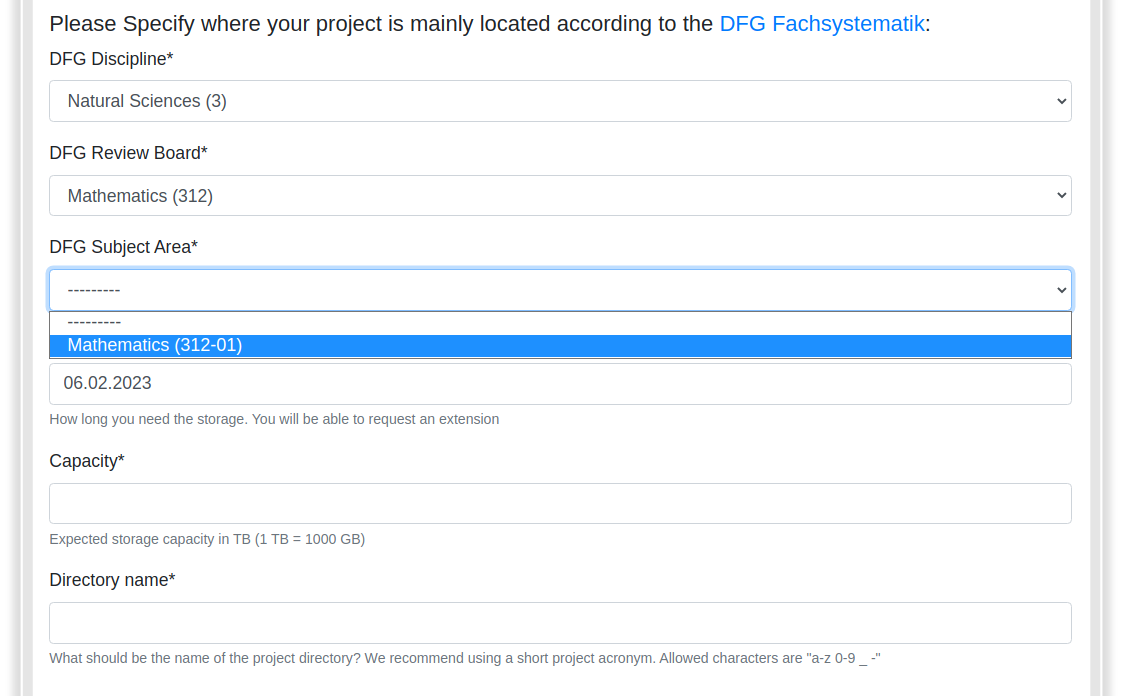
\includegraphics[width=\textwidth]{select_subject2}
\end{frame}


\begin{frame}[c,fragile]{Code Requesting Fields for Boards}
    \footnotesize
    \inputminted[linenos=true]{javascript}{code/board_request.js}
\end{frame}


\begin{frame}[c,fragile]{Backend answering with available Fields}
\footnotesize
    \begin{minted}[linenos]{python}
## urls.py
path('ajax/fields/', views.view_science_fields, name="ajax_load_fields"),

## views.py
def view_science_fields(request):
    b_pk = request.GET.get('board')  # we get the pk of the selected board
    if b_pk:  # select available Fields from this Board
        fields = Science_Field.objects.filter(board__pk=b_pk) 
        return render(request, 'dropdown_list_options.html',
                      {'options': fields})
    return render(request, 'dropdown_list_options.html',
                  {'options': Science_Field.objects.none()})
\end{minted}
\end{frame}

\subsection{Diff csv to DFG schema in database}

\begin{frame}[c]{The DFG schema changes frequently}
    \large
    \begin{itemize}[<+(1)->]
        \item The DFG schema changes every four years
        \item It was last changed in 2020
        \item So it'll change again in two years
        \item Not clear how much (probably not a whole lot)
    \end{itemize}
    \pause
    So I implemented a command to compare any csv to what is currently in the
    database: \mintinline{bash}{manage.py dfg_schema_diff}
\end{frame}


% \begin{frame}[fragile]{Usage of \texttt{dfg_schema_diff}}
\begin{frame}[fragile]{Usage of \texttt{dfg\_schema\_diff}}
    \scriptsize
\begin{verbatim}
usage: manage.py dfg_schema_diff [-h] [--locale LOCALE] [--columns COLUMNS]
                     ...
                     FILE

Show difference from given file schema to DFG schema in database. By default,
ignores the now deprecated hierarchy level 1. ...

positional arguments:
  FILE                  Path to dfg_systematic.csv

options:
  -h, --help            show this help message and exit
  --locale LOCALE       Set the language of the name column to select. Can correctly select
                        both '<locale>' and 'prefLabel@<locale>' columns. (Default: 'en')
  --columns COLUMNS     Dictionary mapping columns (numbers) to expected values "level" (in
                        the hierarchy, category: 0, deprecated/ignored: 1, board: 2, field:
                        3), "notation" (e.g. 101-27), and locale translations, e.g. "en"
                        (double quotes are important!). Defaults to auto.
  ...                   ...
\end{verbatim}
\end{frame}

% \subsection{Rename Models}
% 
% \begin{frame}[c]
%     % Order -> LSDFProject
%     % PersonOrder -> ProjectRole
%     % ...
%     Worked quite well, generated some migrations
% \end{frame}

% \subsection{Attempt to rename entire App}
% 
% \begin{frame}[c]
%     Failed, ultimately unclear why, requires deep django/database knowledge.
% \end{frame}


\subsection{Attempt to properly modularize PersonForm}

\begin{frame}[c]
    Explain the problem (show exemplary code) of redundancy
    Managed to get quite far, very good (deep) learning example, and absolutely
    possible. just requires some more time than expected.
    Nags me that it's not modular yet. Some day.
\end{frame}


\subsection{Extension Requests}

\begin{frame}[c]
    WHY Extension Requests
\end{frame}

\begin{frame}[c]{Extension Requests}
    Much-requested feature.
    \todo{Overview of newly introduced routes, views, forms, models and relations}
\end{frame}
